\chapter{Explanation of the Mobile Application}

\section{The Building Blocks}



The following sections will explain integral parts of the server and client part of the mobile application. A gist of the architecture is shown
in figure \ref{fig:bb}. As it can be seen, the mobile app represents the user participating in the experiment. As the experiment goes on,
mobile sensor data and responses to the data requests which are collected are periodically sent to the Kinvey Data Store. 
The users can choose to login into the FairDataShare Portal from their computer or the mobile app. Once the user is authenticated, the user request
is sent from the FairDataShare server to the Kinvey Data Store. Kinvey in turn fetches the appropriate data and gives it to the FairDataShare Server. This in turn structures the data so it can be easily readable, and pushes it to the user to see on the portal. The concept is similar for the Stakeholders, except they can only access the portal through the computer and not the mobile app.

\begin{figure}[ht!]
\centering
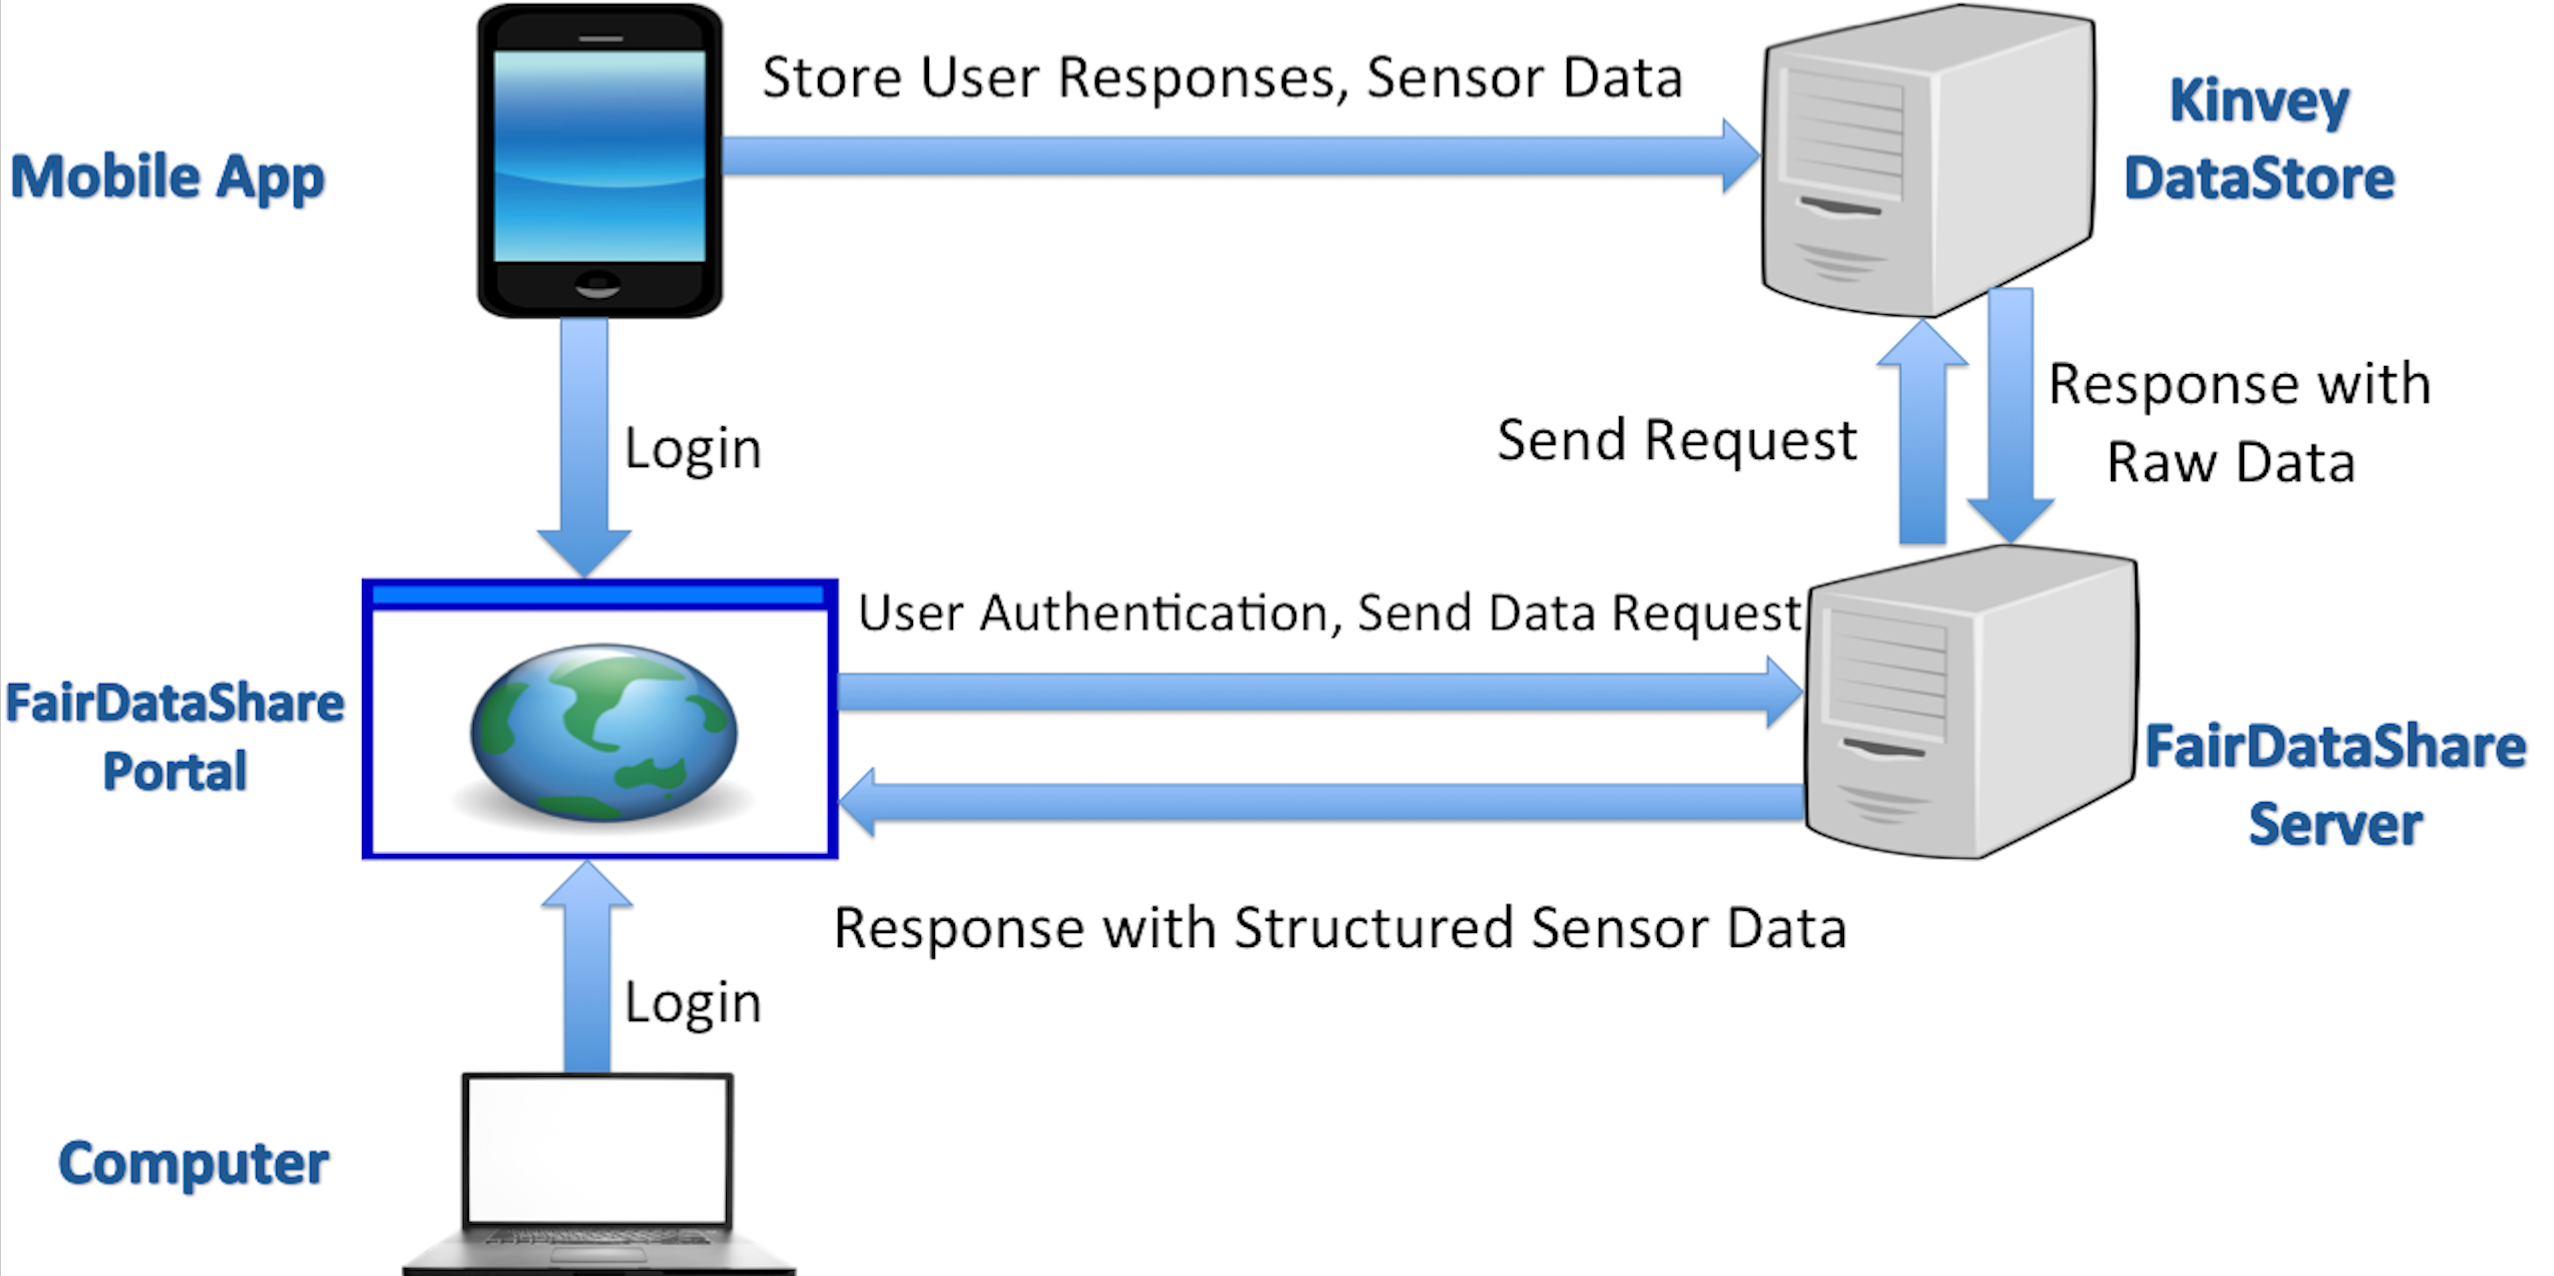
\includegraphics[width=\textwidth,keepaspectratio]{./images/blocks_app}
\caption{Conceptual Diagram of Mobile Application Architecture}
\label{fig:bb}
\end{figure}


\section{The Mobile Application}





\subsection{Local Storage}
The local storage is an integral part of the application. The database used is SQLite and is the default database
for the Android environment. Small sized unrelated data is stored in preferences files, whereas larger related
data is stored in the database. The following paragraphs will explain each database present in this application followed with 
their function. All tables explained here are pertaining to the user using the mobile application.

\begin{figure}[htp]
\subtop[Table Schema of QUESTIONSTORE\label{fig:db_quest}]{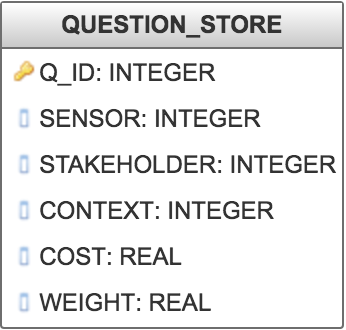
\includegraphics[width=0.4\linewidth]{./images/db_quest}}\hspace{1em}
\subtop[Table Schema of WHICHANSWERS\label{fig:db_which}]{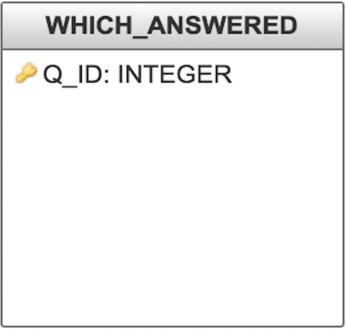
\includegraphics[width=0.4\linewidth]{./images/db_which_1}}
\caption{Table Schemas}
\label{fig:ts1}
\end{figure}


Figure \ref{fig:db_quest} shows the QUESTIONSTORE's table schema. This table stores each possible data request with its sensor $SENSOR$, stakeholder  $STAKEHOLDER$ and context $CONTEXT$. Each of these are represented by an integer, for example sensor 0 stands for Accelerometer sensor. Each data request is accompanied by
an unique question identifier $QID$, weight assigned $WEIGHT$ and the cost $COST$. This data is not sent to 
the server.

Figure \ref{fig:db_which} depicts the table WHICHANSWERS's table schema. This stores the questions identifier $QID$ of each data request that has
been answered by the user for each round. This is helpful while fetching data requests, so as not to fetch the request twice in the same round. This makes sure that all questions are answered before answering them for a second time. This data is not sent to the server.

\begin{figure}[htp]
\subtop[Table Schema of STOREANSWERS\label{fig:db_ans}]{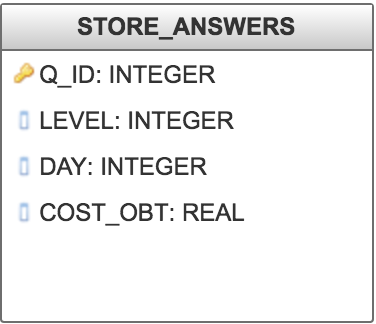
\includegraphics[width=0.4\linewidth]{./images/db_ans}} \hspace{1em}
\subtop[Table Schema of STOREPOINTS\label{fig:db_points}]{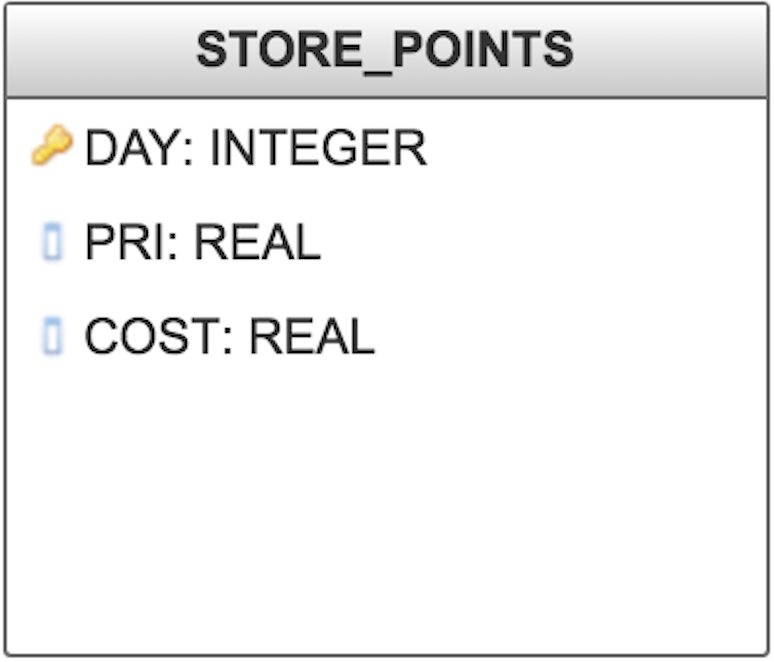
\includegraphics[width=0.4\linewidth]{./images/db_points}}
\caption{Table Schemas}
\label{fig:ts11}
\end{figure}

Figure \ref{fig:db_ans} explains the schema of STOREANSWERS table. This table is used to store the data request identifier $QID$ with the corresponding
user responses $LEVEL$, along with the increase or decrease in credit obtained $COST_OBT$. The total cost can be calculated by adding all the costs in this table. Similarly, the total privacy can be calculated by averaging all the user responses in this table. Only the most recent responses are stored in this table. This content is not sent over to the server.

Figure \ref{fig:db_points} denotes the schema of STOREPOINTS table. This table is used to store the credit and privacy obtained for each bidding day.
This information is sent to the server as soon one bidding day is over.

\begin{figure}[ht!]
\centering
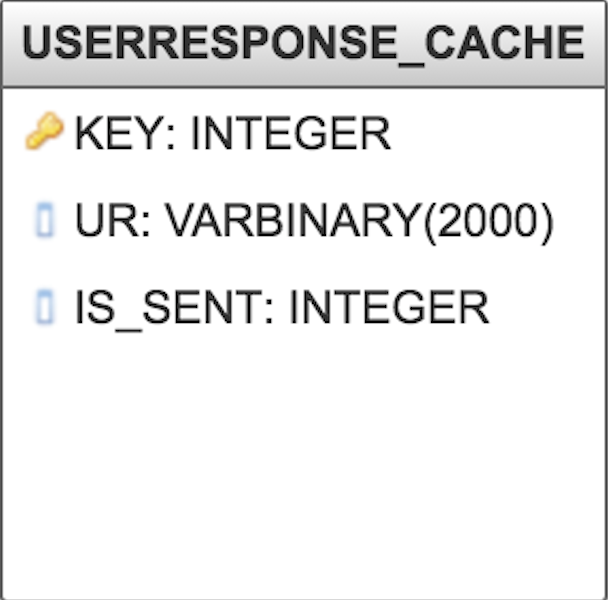
\includegraphics[width=0.4\linewidth]{./images/db_ur}
\caption{Table USERRESPONSECACHE Schema}
\label{fig:db_ur}
\end{figure}

Figure \ref{fig:db_ur} depicts the USERRESPONSECACHE tables's schema. This table stores a unique key $KEY$ for each user response, followed by a flag $ISSENT$, which is 1 if the response is not sent to the server, and 0 if it is sent. The user response saved consists of the following entries :

\begin{enumerate}
	\item User Id
	\item Timestamp of response
    \item Sensor Id
    \item Stakeholder Id
    \item Context Id
    \item Privacy Level answered for this data request
    \item Cost obtained for this data request
    \item Current Total Privacy of user
    \item Current Total Credit of user
    \item Maximum Obtainable Credit for this data request in this round
    \item Metric Chosen to Improve  (Improve Privacy or Improve Credit)
\end{enumerate}

All of the above fields are packed into the field $ur$ shown in \ref{fig:db_ur}. The data in this table is sent to the server. Once the entry is sent to the server, the $ISSENT$ field is changed to 0 and deleted locally. The unique keys $KEY$ are useful for deleting sent entries.

Figure \ref{fig:ts2} and \ref{fig:ts22} show the table schemas for data storage of the following sensors:

\begin{enumerate}
	\item Accelerometer in the STOREACCELEROMETER table
	\item Noise in the STORENOISE
    \item Location in the  STORELOCATION
    \item Light in the  STORELIGHT
\end{enumerate}

\begin{figure}[htp]
\subtop[Table Schema of STOREACCELEROMETER\label{fig:db_acc}]{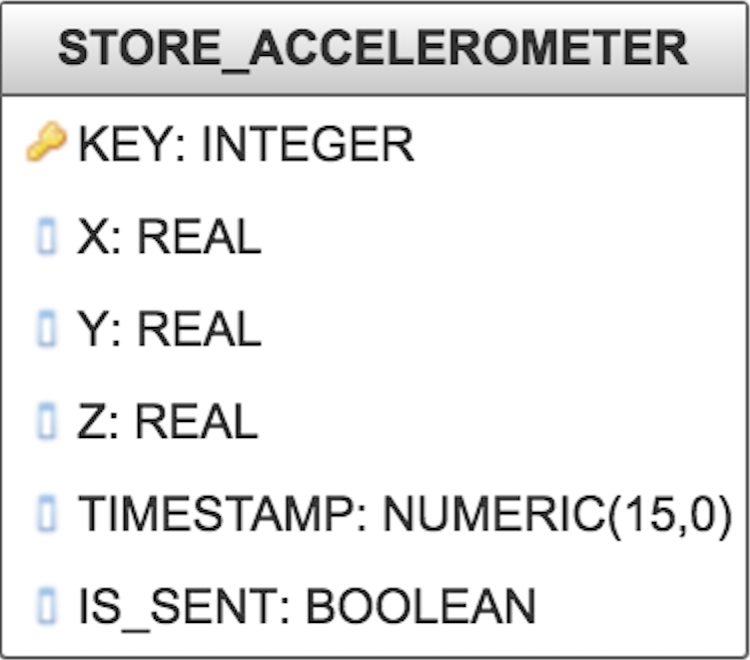
\includegraphics[width=0.4\linewidth]{./images/db_acc}}\hspace{1em}
\subtop[Table Schema of STORENOISE \label{fig:db_noise}]{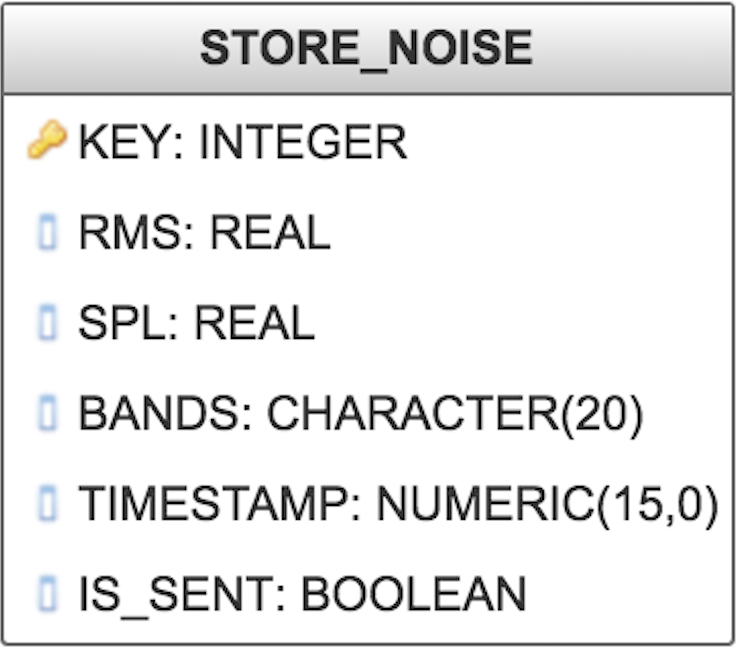
\includegraphics[width=0.4\linewidth]{./images/db_noise}}%
\caption{Table Schemas for Sensor Data}
\label{fig:ts2}
\end{figure}

The general schema for all the sensors is the following :

\begin{enumerate}
	\item $KEY$ - Uniquely identifies each sensor entry
	\item $TIMESTAMP$ - The time the sensor value was collected
    \item $ISSENT$ - Denotes whether the sensor entry has been sent to the server or not
    \item The other columns are specific to each sensor and represent the actual sensor values of the user collected
\end{enumerate}

\begin{figure}[htp]
\subtop[Table Schema of STORELOCATION\label{fig:db_loc}]{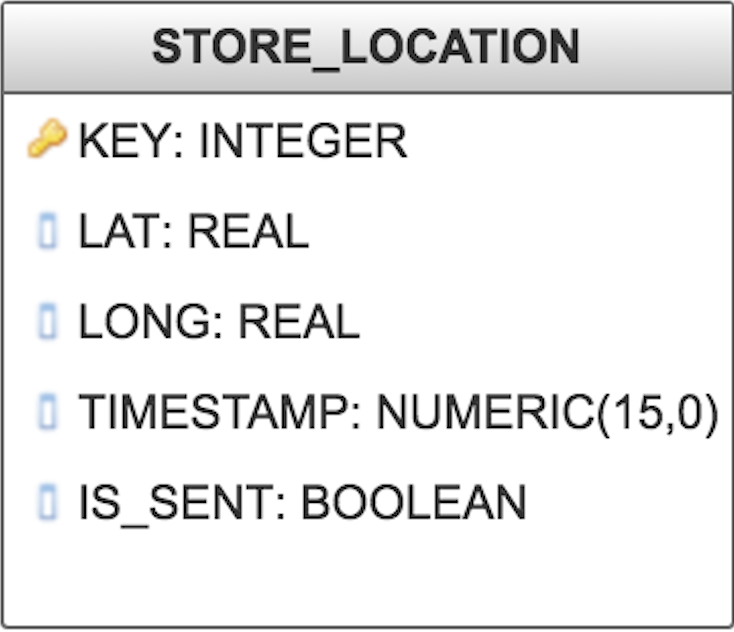
\includegraphics[width=0.4\linewidth]{./images/db_loc}}\hspace{1em}
\subtop[Table Schema of STORELIGHT \label{fig:db_light}]{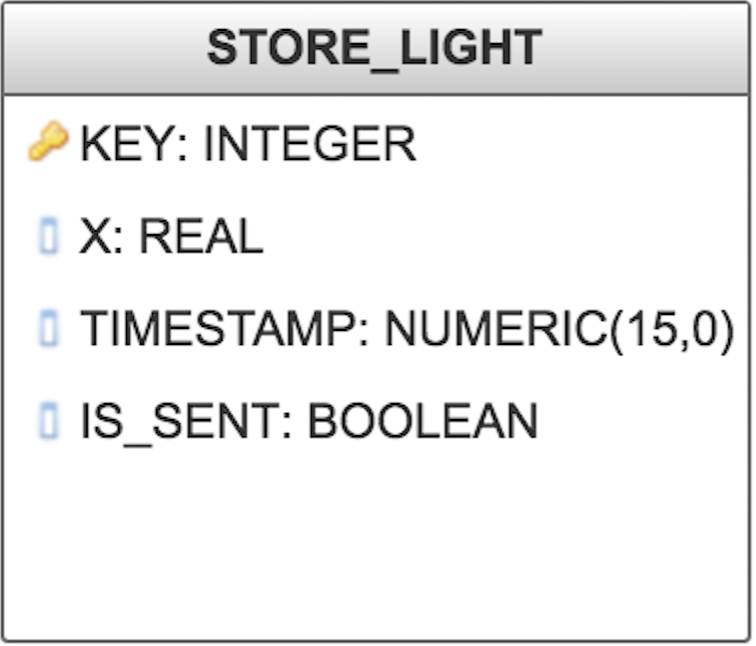
\includegraphics[width=0.4\linewidth]{./images/db_light}}%
\caption{Table Schemas for Sensor Data}
\label{fig:ts22}
\end{figure}


\subsection{Alarms and Notifications}

Every bidding day where the user can answer data requests lasts for a period of 24 hours. After one bidding day is over, the system needs to be informed in a timely to perform some application critical functions. The function performed are explained in detail in section \ref{next}. 
To inform the system of such an event Android provides the functionality in the form of alarms. Alarms can be set to go off just once or in a repeated fashion to trigger tasks. Unfortunately, the alarms provided by Android are not exact for some versions, in the sense that they are triggered around that time set but not exactly to optimize the battery. Hence, we decided to set the repeating alarms manually. The first time the alarm is set to ring in exactly 24 hours, but things change when the phone is switched off.


One of the conditions of the experiment is not to have the phone switched off at any time. Neverthless, we take into account the scenario where
the phone is kept switched off for a period of time. There are various things that can happen:

\begin{enumerate}
	\item The phone is rebooted.
	\item The phone is switched off, during this time an alarm is missed.
    \item The phone is switched off for a period greater than 24 hours. One or more alarms can be missed.
\end{enumerate}

Once the phone is switched off, all alarms are erased. Alarms do not execute when the phone is switched off. Hence, when the phone switches on,
BootReceiver service of the application is triggered with pseudocode \ref{boot}.

\begin{algorithm}
\caption{BootService Algorithm}\label{boot}
\begin{algorithmic}[1]
\Procedure{BootService}{}
\State $\textit{now} \gets \text{current timestamp}$
\State $i \gets \text{timestamp of last triggered alarm}$
\If {$\textit{now}-i < 86400$}
  \State $\text{Call }\textit{SetAlarmLater()}$
\Else
  \State $\text{Set alarm in 200 seconds}$
\EndIf
\EndProcedure
\end{algorithmic}
\end{algorithm}



\begin{algorithm}
\caption{Alarm Algorithm}\label{setalarm}
\begin{algorithmic}[1]
\Procedure{SetAlarmLater}{}
\State $\textit{now} \gets \text{current timestamp}$
\State $i \gets \text{timestamp of last triggered alarm}$
\State $\textit{latertime} \gets \textit{i}+\text{86400}$
\State $\textit{latergap} \gets \textit{latertime}-\textit{now}$
\State $\text{Set Alarm in latergap seconds}$
\EndProcedure
\end{algorithmic}
\end{algorithm}

\subsubsection{Going to the Next Data Sharing Day} \label{next}
When the alarm notifies the system that one bidding day is over, 

\begin{algorithm}
\caption{NextDayService Algorithm}\label{nextday}
\begin{algorithmic}[1]
\Procedure{NextDayService}{}
\State $\text{Store }\textit{Privacy, Credit, Day } \text{in } \textit{STOREPOINTS}$
\State $\text{Send }\textit{Privacy, Credit, Day } \text{to Server}$
\State $\textit{Privacy, Credit, Round, CurrentQuestion} \gets \text{0}$
\State $\textit{Day} \gets \textit{Day}+1$
\State $\text{Store current time}$
\State $\text{Call }\textit{Summarization()}$
\If {$\textit{Day} > \textit{End}$}
  \State $\text{End experiment}$
\Else
  \State $\text{Update user interface elements}$ 
\EndIf
\EndProcedure
\end{algorithmic}
\end{algorithm}


\subsection{Fetching Data Requests}




\subsection{Recording User Choices}

\subsection{Sensor Data Collection and Summarization}

\begin{algorithm}
\caption{Summarization Algorithm}\label{sum}
\begin{algorithmic}[1]
\Procedure{Summarization}{}
\For{$\text{each sensor}$}
\State $\text{Fetch sensor data from } \textit{sensor table}$
\State $\textit{level} \gets \text{Fetch user privacy level}$
\If {$\textit{level} \gets 1$}
  \State $\text{Set all } \textit{ISSENT} \gets \text{1}$
\ElsIf {$\textit{level} \gets 2$}
	\For{$\text{3 out of every 4 records}$}
 	 \State $\textit{ISSENT} \gets \text{1}$
 	\EndFor 
\ElsIf {$\textit{level} \gets 3$}
  \For{$\text{1 out of every 2 records}$}
 	 \State $\textit{ISSENT} \gets \text{1}$
 	\EndFor
\ElsIf {$\textit{level} \gets 4$}
  \For{$\text{1 out of every 4 records}$}
 	 \State $\textit{ISSENT} \gets \text{1}$
 	\EndFor
\EndIf
\State $\text{Delete all entries with } \textit{ISSENT} \gets 0$
\State $\text{Update Database}$
\EndFor
\EndProcedure
\end{algorithmic}
\end{algorithm}

\subsection{Server Synchronization}
\begin{algorithm}
\caption{NetworkService Algorithm}\label{nextday}
\begin{algorithmic}[1]
\Procedure{NetworkService}{}
\State $ \text{Fecth data from } \textit{USERRESPONSECACHE}$
 \For{$\text{each record}$}
 	 \If {$\textit{ISSENT} == \textit{1}$}
  \State $\text{Send record to Server}$
\Else
  \State $\text{Delete record}$ 
  \EndIf
 	\EndFor

\For{$\text{each sensor}$}
 	 \State $ \text{Fecth data from } \textit{sensor table}$
 	  \For{$\text{each record}$}
 	 \If {$\textit{ISSENT} == \textit{1}$}
  \State $\text{Send record to Server}$
	\Else
  \State $\text{Delete record}$
  \EndIf
 	\EndFor
	
 	\EndFor
\EndProcedure
\end{algorithmic}
\end{algorithm}



\subsubsection{Going to the Next Data Sharing Day} \label{next}



\section{The Server}

\subsection{Kinvey Data Storage}

Kinvey is a mobile backend as a service which provides a platform for mobile phones to link applications at a backend cloud storage. This backend has been used to store data and for some business logic implementations.
\subsubsection{Security}

\subsubsection{Table Store}

\begin{figure}[ht!]
\centering
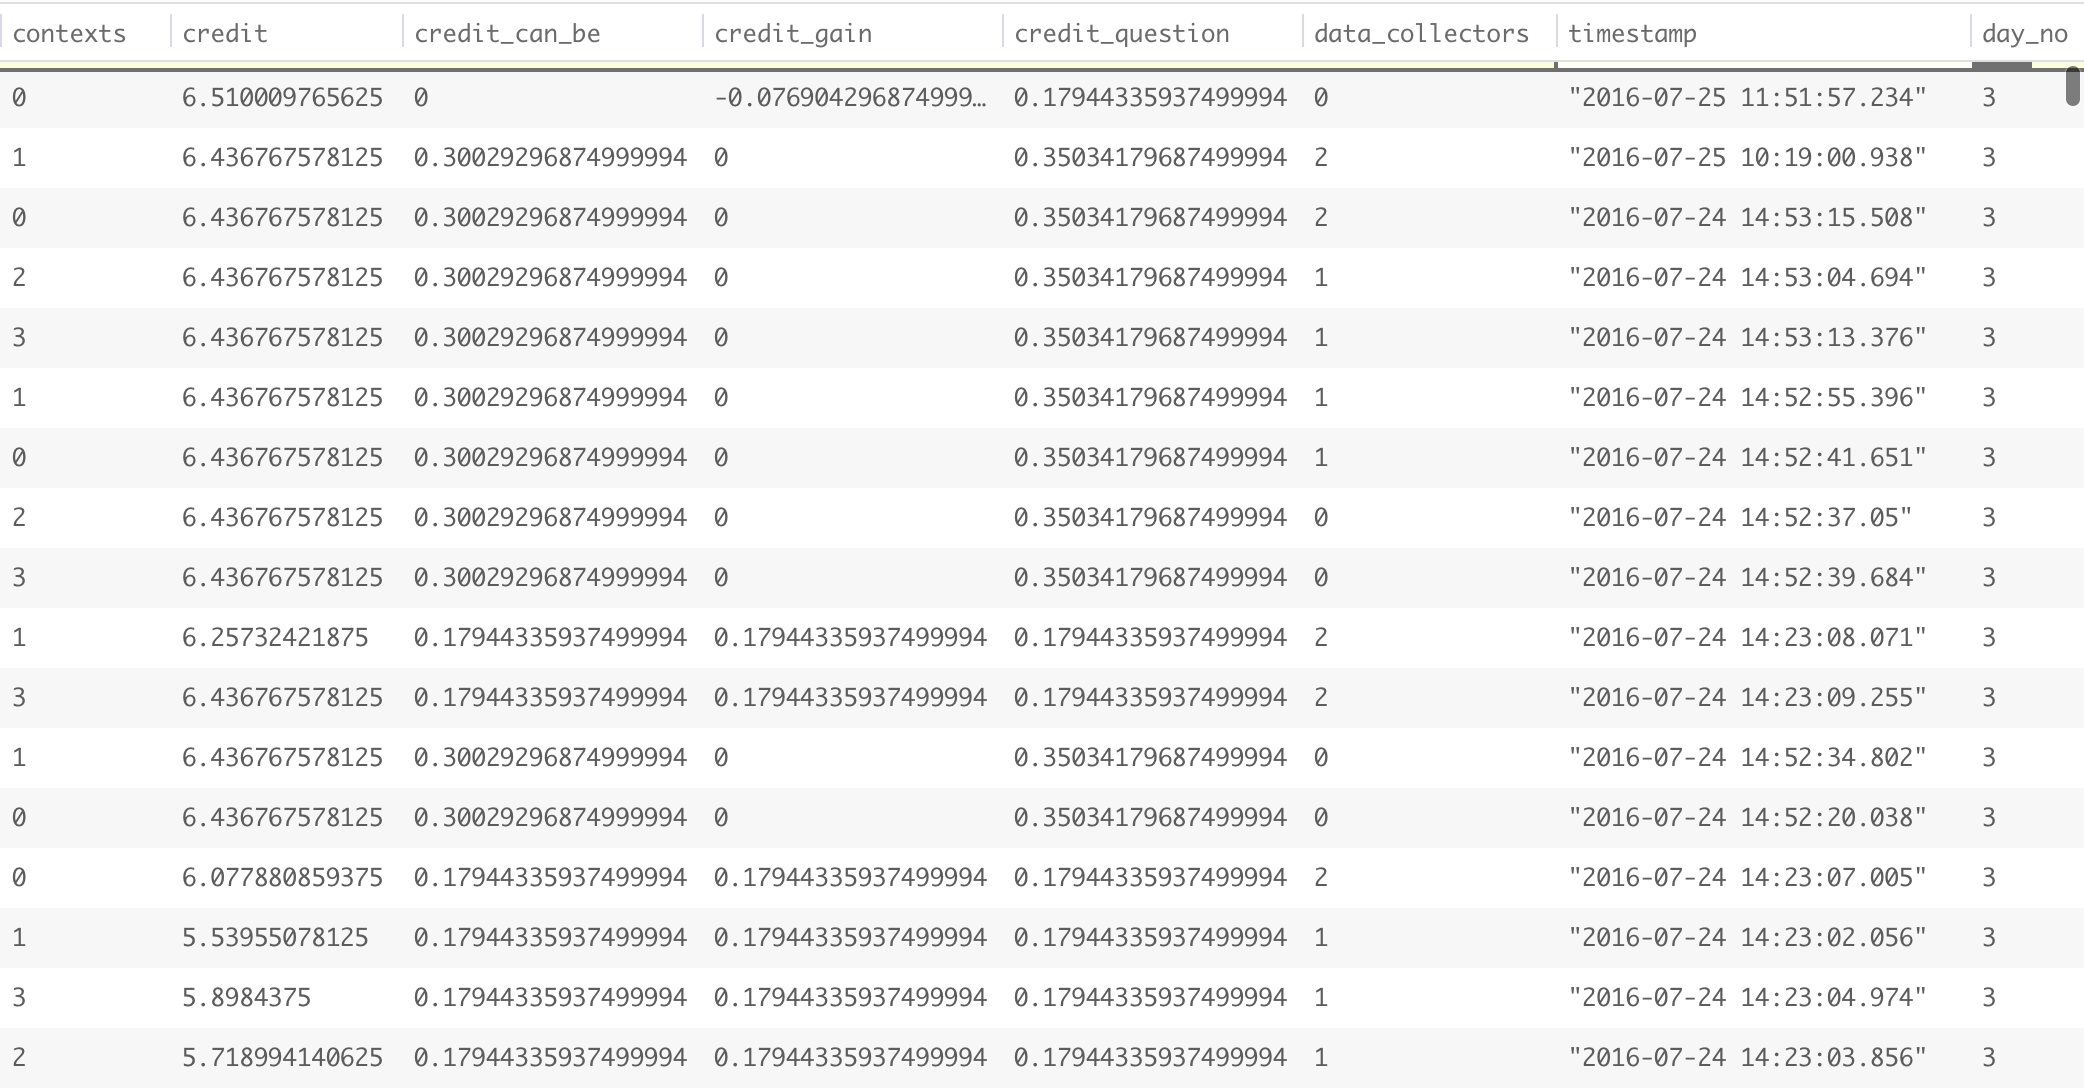
\includegraphics[width=\textwidth,keepaspectratio, height=0.6\textwidth]{./images/collection_ur_1}
\caption{Screenshot of Collection UserResponse Part 1}
\label{fig:col_ur_1}
\end{figure}

\begin{figure}[ht!]
\centering
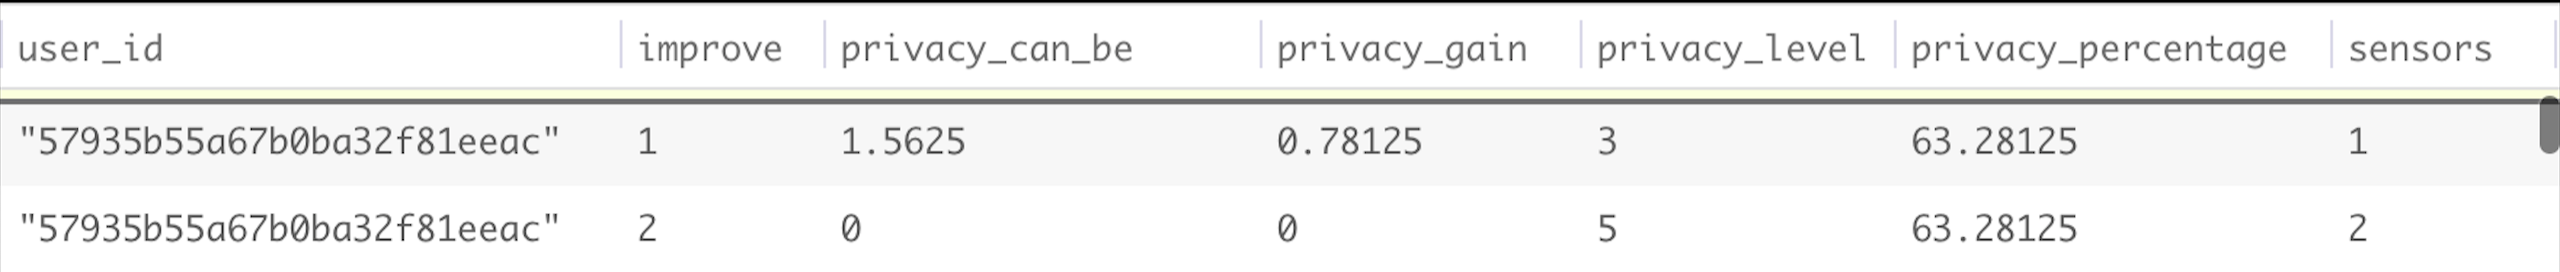
\includegraphics[width=\textwidth,keepaspectratio,height=0.6\textwidth]{./images/collection_ur_2}
\caption{Screenshot of Collection UserResponse Part 2}
\label{fig:col_ur_2}
\end{figure}

\begin{figure}[ht!]
\centering
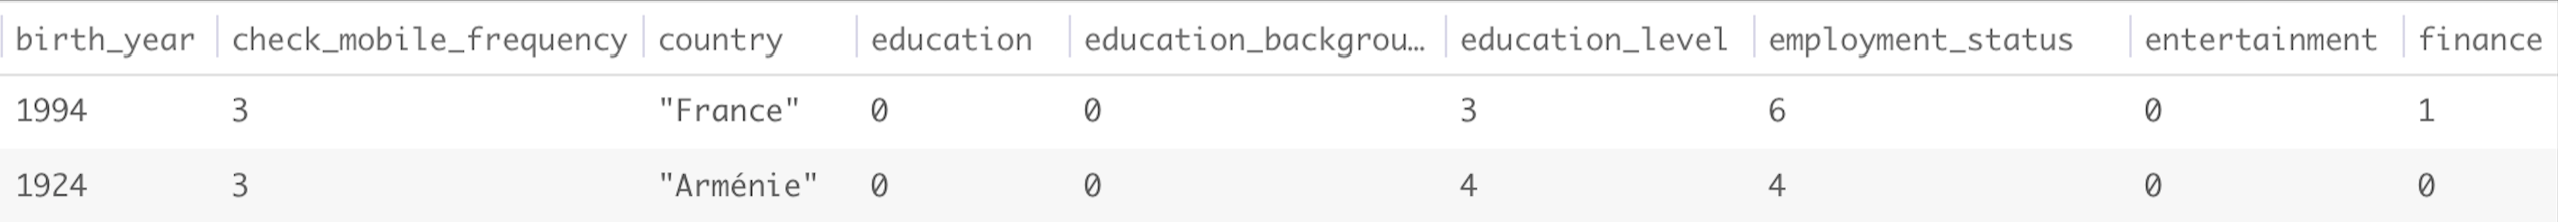
\includegraphics[width=\textwidth,keepaspectratio,height=0.6\textwidth]{./images/collection_ui_1}
\caption{Screenshot of Collection UserInformation Part 1}
\label{fig:col_ui_1}
\end{figure}

\begin{figure}[ht!]
\centering
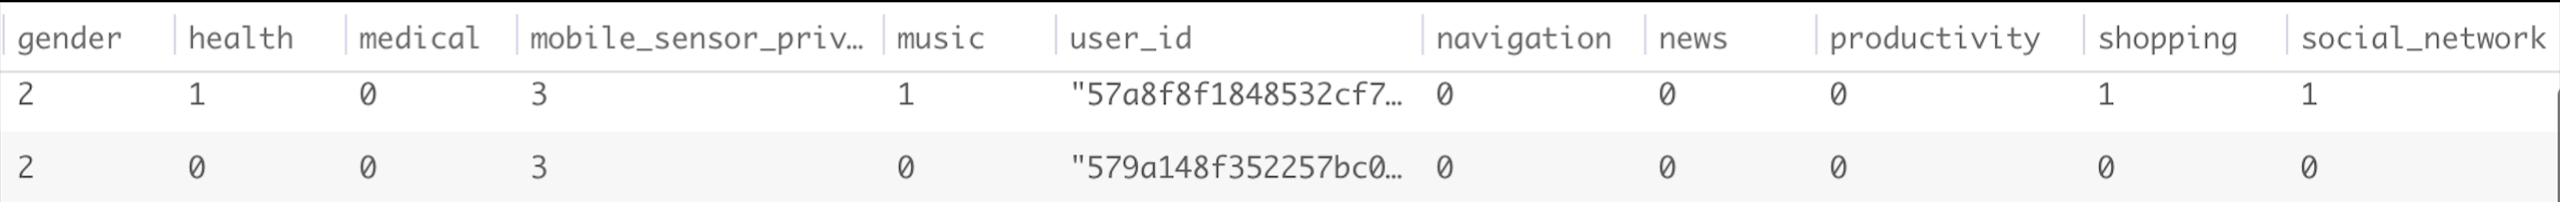
\includegraphics[width=\textwidth,keepaspectratio,height=0.6\textwidth]{./images/collection_ui_2}
\caption{Screenshot of Collection UserInformation Part 2}
\label{fig:col_ui_2}
\end{figure}

\begin{figure}[ht!]
\centering
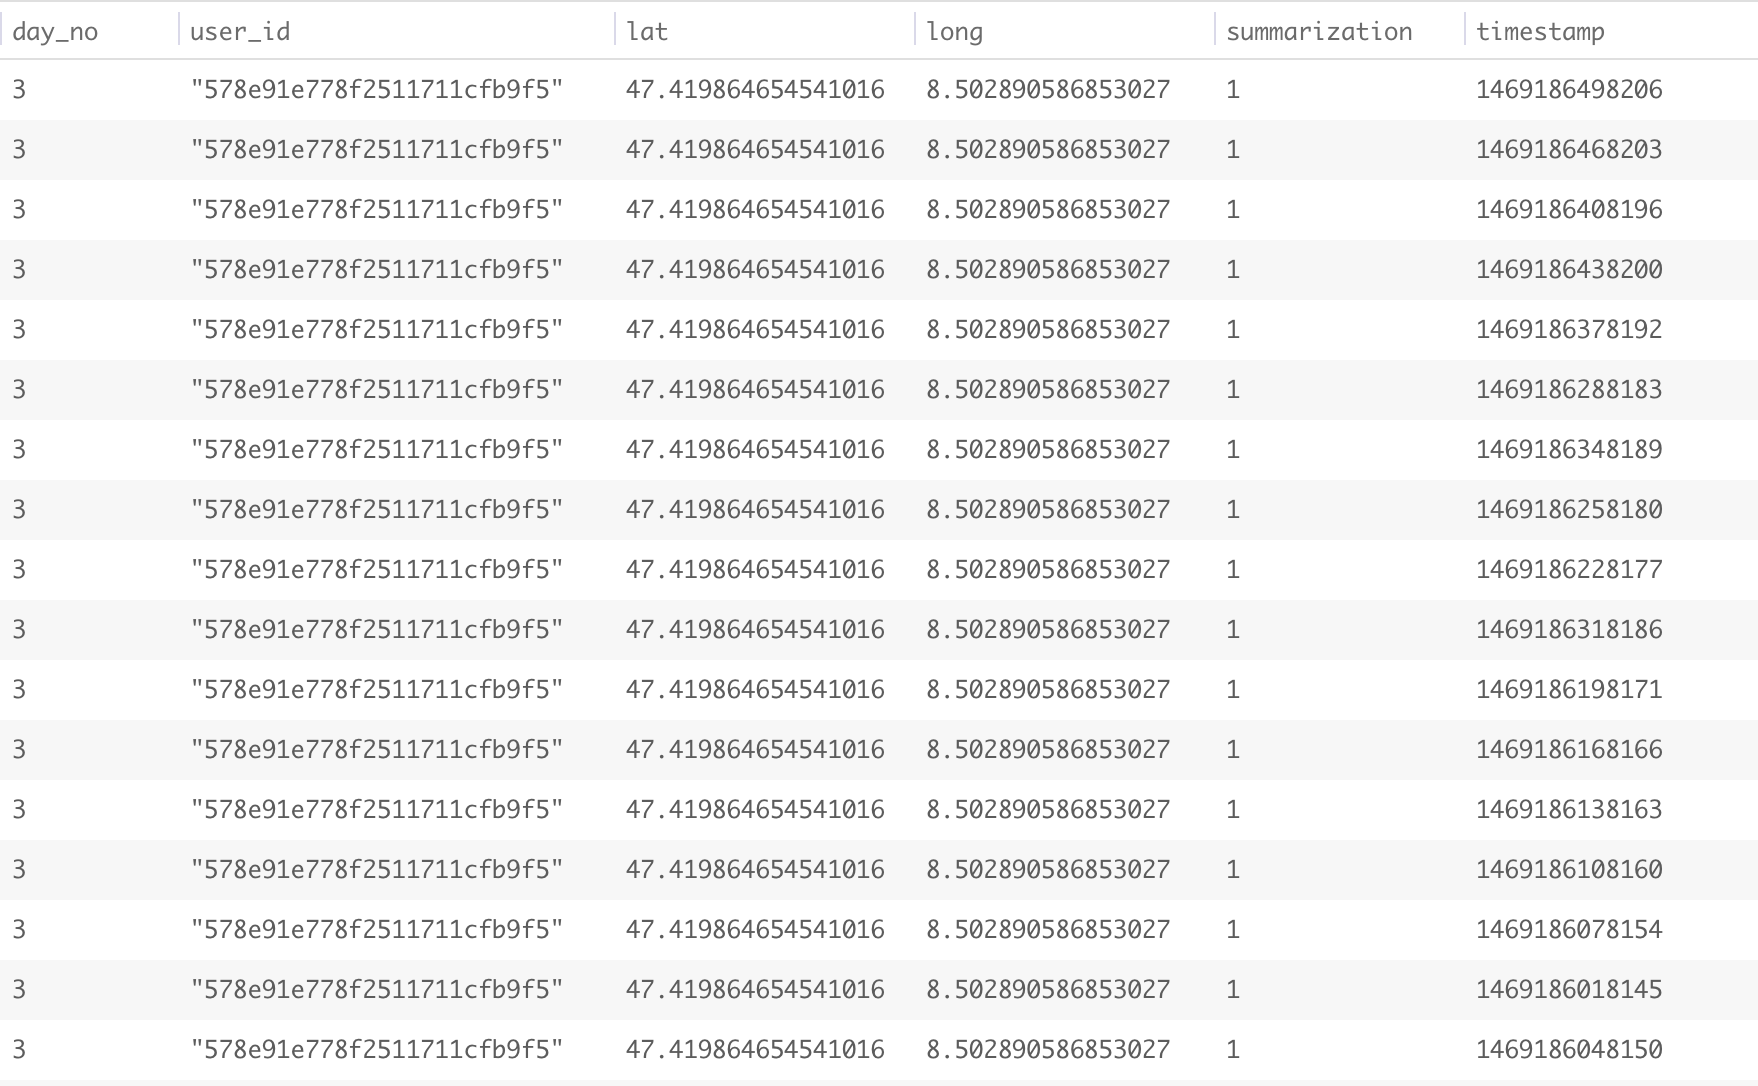
\includegraphics[width=\textwidth,keepaspectratio,height=0.6\textwidth]{./images/collection_loc}
\caption{Screenshot of Collection Location}
\label{fig:col_loc}
\end{figure}

\begin{figure}[ht!]
\centering
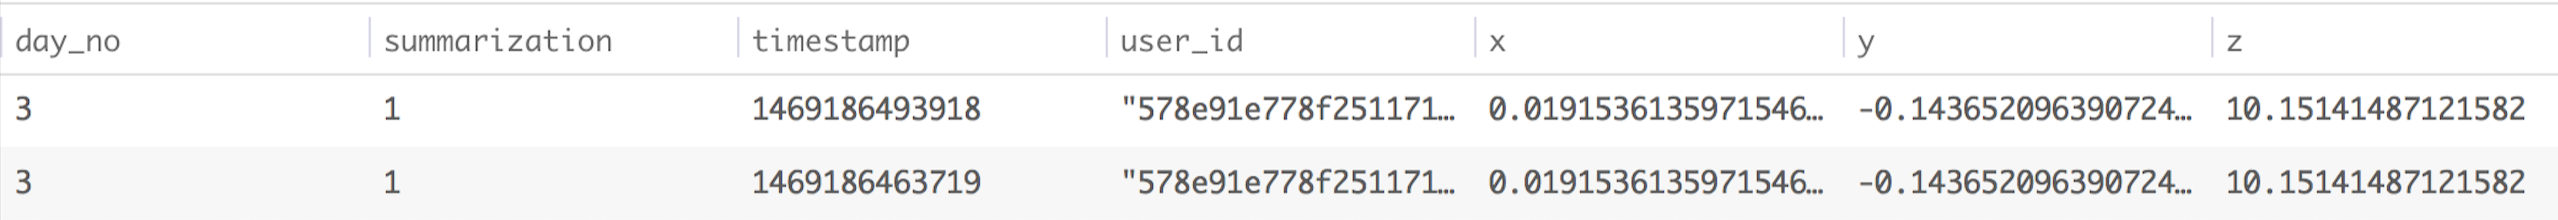
\includegraphics[width=\textwidth,keepaspectratio,height=0.6\textwidth]{./images/collection_acc}
\caption{Screenshot of Collection Accelerometer}
\label{fig:col_acc}
\end{figure}

\begin{figure}[ht!]
\centering
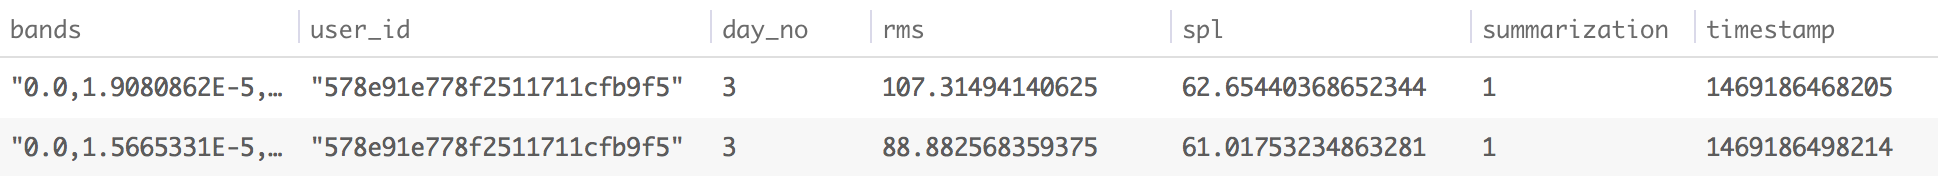
\includegraphics[width=\textwidth,keepaspectratio,height=0.6\textwidth]{./images/collection_noise}
\caption{Screenshot of Collection Noise}
\label{fig:col_noise}
\end{figure}

\begin{figure}[ht!]
\centering
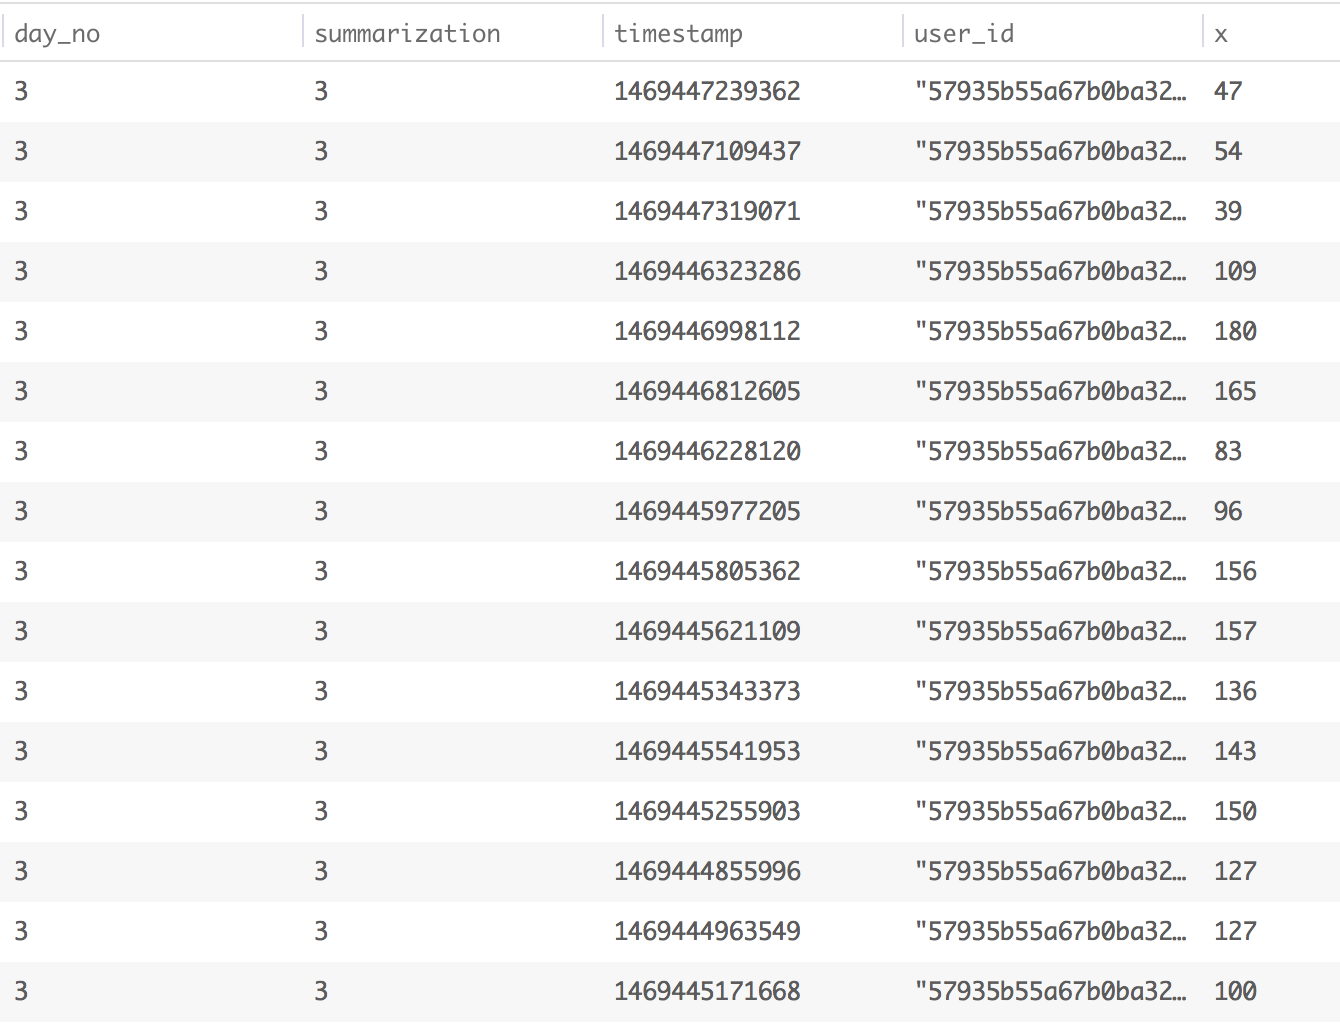
\includegraphics[width=\textwidth,keepaspectratio,height=0.6\textwidth]{./images/collection_light}
\caption{Screenshot of Collection Light}
\label{fig:col_light}
\end{figure}

\begin{figure}[ht!]
\centering
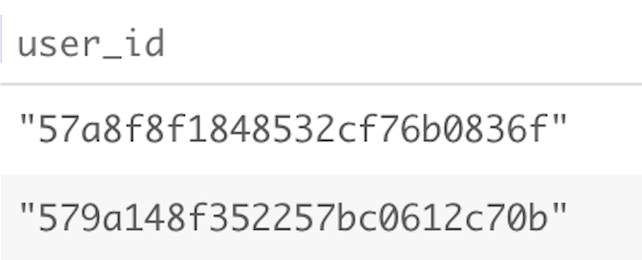
\includegraphics[width=\textwidth,keepaspectratio,height=0.6\textwidth]{./images/collection_users}
\caption{Screenshot of Collection Users}
\label{fig:col_users}
\end{figure}

\begin{figure}[ht!]
\centering
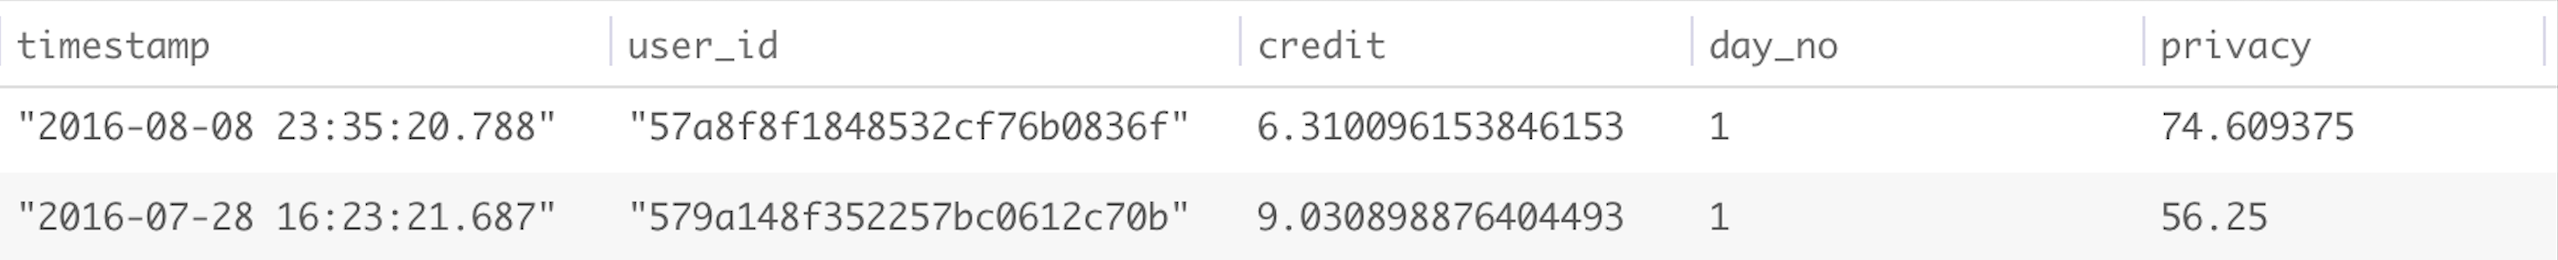
\includegraphics[width=\textwidth,keepaspectratio,height=0.6\textwidth]{./images/collection_score}
\caption{Screenshot of Collection Score}
\label{fig:col_score}
\end{figure}

\begin{figure}[ht!]
\centering
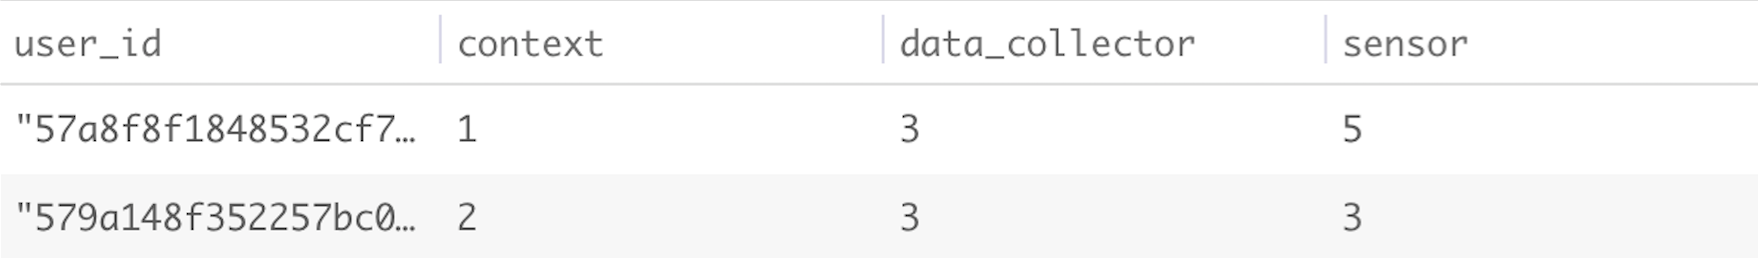
\includegraphics[width=\textwidth,keepaspectratio,height=0.6\textwidth]{./images/collection_feature_cat}
\caption{Screenshot of Collection Features}
\label{fig:col_f}
\end{figure}

\begin{figure}[ht!]
\centering
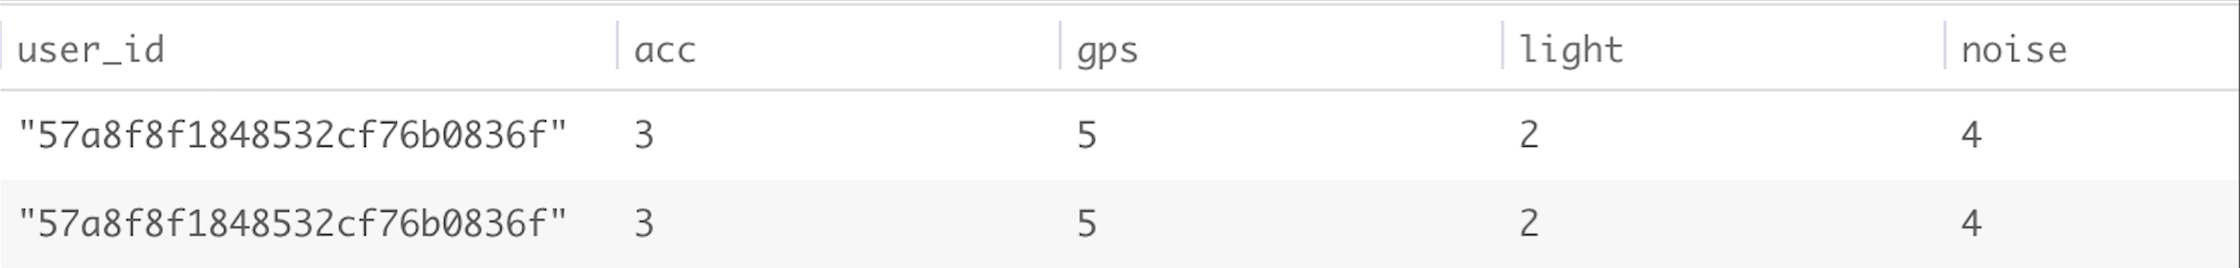
\includegraphics[width=\textwidth,keepaspectratio,height=0.6\textwidth]{./images/collection_sensors_cat}
\caption{Screenshot of Collection Sensors}
\label{fig:col_s}
\end{figure}

\begin{figure}[ht!]
\centering
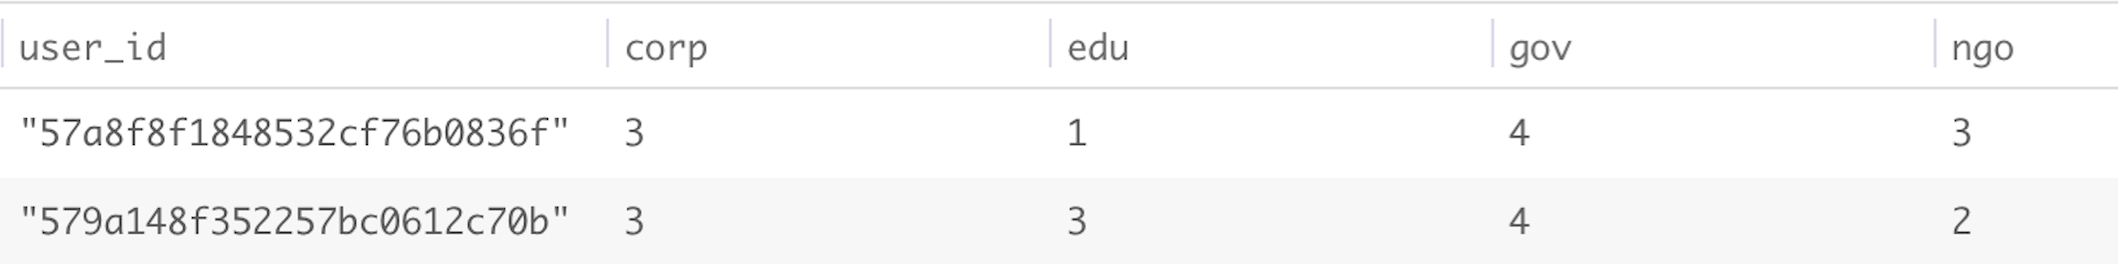
\includegraphics[width=\textwidth,keepaspectratio,height=0.6\textwidth]{./images/collection_dc_cat}
\caption{Screenshot of Collection Stakeholders}
\label{fig:col_ss}
\end{figure}

\begin{figure}[ht!]
\centering
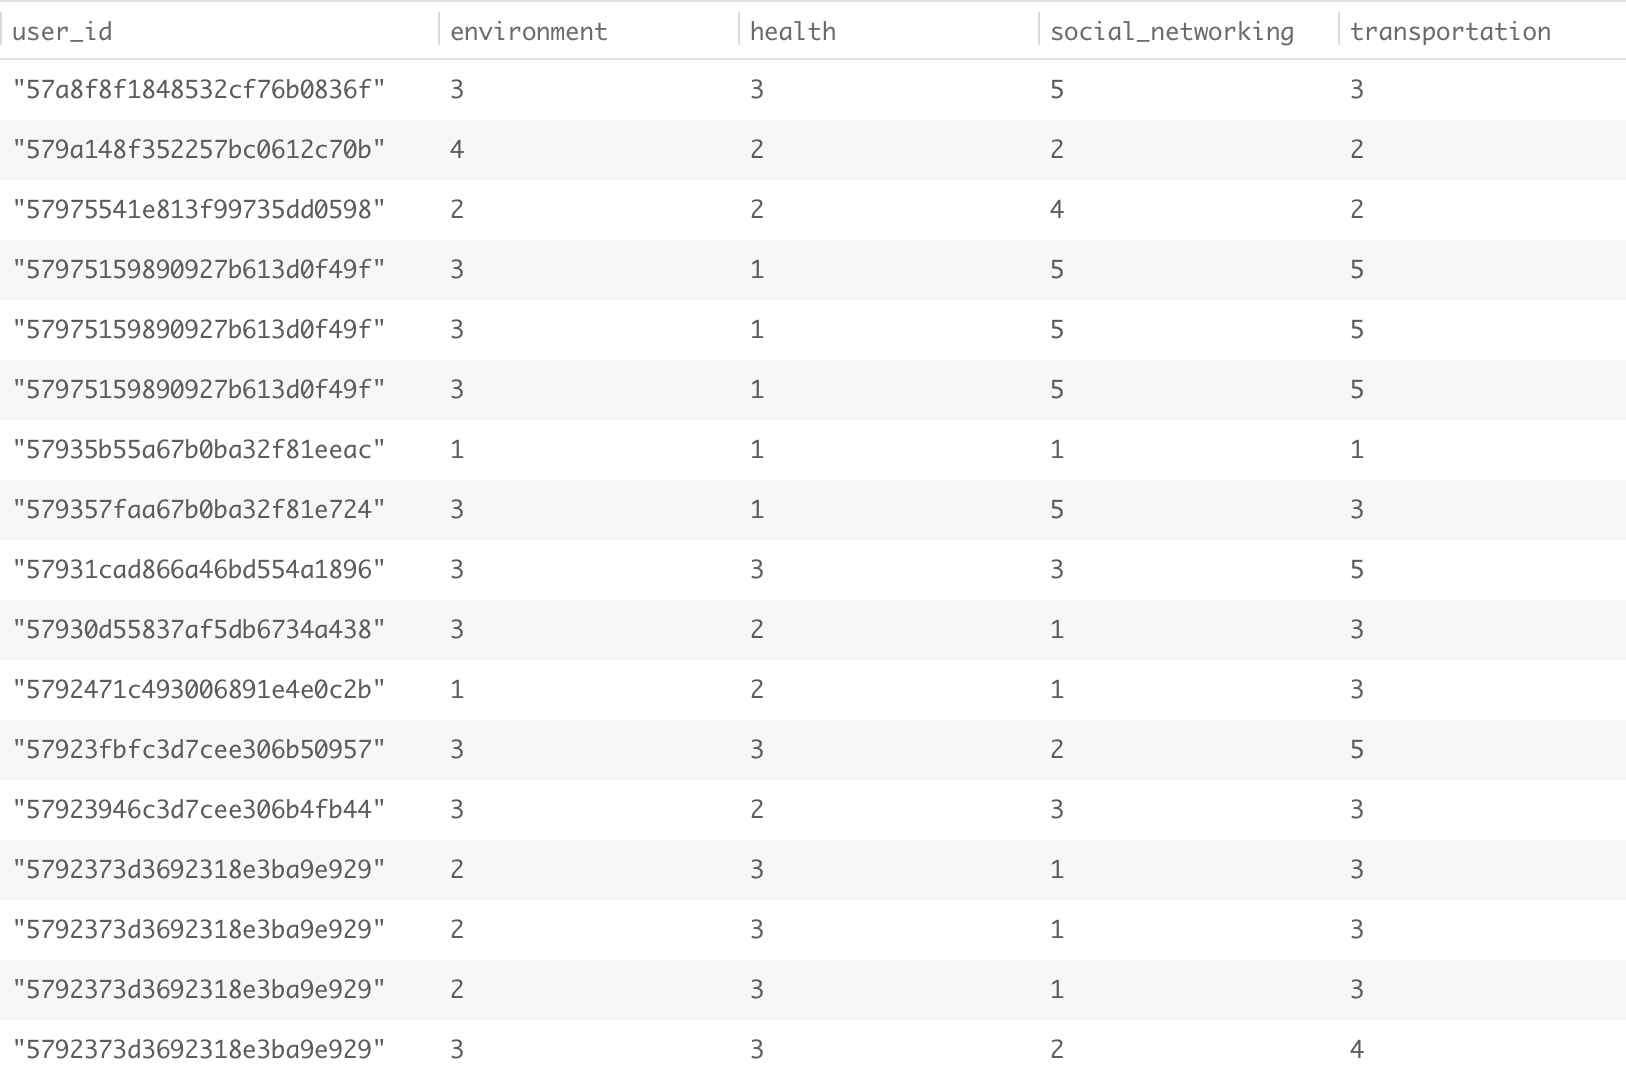
\includegraphics[width=\textwidth,keepaspectratio,height=0.6\textwidth]{./images/collection_context_cat}
\caption{Screenshot of Collection Contexts}
\label{fig:col_c}
\end{figure}

All the data collected form the user's phones is stored in Kinvey Data Store's collections. Data is segregated in to the appropriate collections. Data is stored in the collections is done so in the following form :

\begin{enumerate}
    \item Data collected in the form of radio buttons on the phone are stored as integers.
    \item Data collected as check-box entries on the phone each have a column in the collection with entries zero or one.
    \item Data collected as drop down lists on the phone are stored either by integer position in the list or by the entry name in the list itself.
\end{enumerate}

This way of storing data applies to all the collections explained below. Each record of every collection is with a unique user identifier and with the timestamp whenever necessary. This is done to identify data that belongs to the same user accross different collections. The timestamp
is collected in order to examine temporal relationships.
The first collection is the GetUserInformation collection and is used to store all the basic non intrusive user information 
collected in the entry phase. The collection is shown in figure \ref{}. Next, is the UserResponse collection which is used to store all
the responses of the users to data requests in the entry phase and the core phase. The collection is shown in figure \ref{}. Collection AccelerometerStore, LightStore, NoiseStore and LocationStore are used to store the mobile sensor data collected from the user at the end of a bidding day after local summarization on the mobile phone. Theses collections are shown in figures \ref{} \ref{} \ref{} \ref{}. The StorePoints collection is used to store the privacy and credit metrics obtained at the end of each bidding day  for each user and is shown in figure \ref{}.

\subsubsection{Bussiness Logic} \ref{bl}
Most of the bussiness logic used in the FairDataShare portal is present on Kinvey. Two things are done here:
\begin{enumerate}
    \item Finding privacy for a user
    \item Summarization
\end{enumerate}
Data collected from the user consists of mobile sensor data with the least amount of summarization. This prevents for repeatedly
collecting data from users and saves space and mobile data. Therefore, this mobile sensor data needs to be further summarized before being given to the stakeholder. To do this, we first have to find the most recent privacy setting from the UserResponseCollection. This is done due to the fact users can answer a data request more than once, hence we need to fish out the latest response for a particular sensor. Once this is done, using the recorded privacy level, we feed this input into another script that performs the summarization which has been explained in chapter \ref{model}.

\subsection{FairDataShare Web Portal}
The FairDataShare portal makes use of a server other Kinvey to safely store the usernames, passwords of users and the stakeholders. The database
technology used is MongoDB. The username and passwords are both stored in a collection. The language used to interact with Kinvey is Express.js, which is based on Node.js. Most of the data portal business logic is on Kinvey described in section \ref{bl}. The webpage was constructed using Html and css. Screenshots of the portal are provided in chapter \ref{exp}.









